En la sección anterior se estudiaron las operaciones en naturales. Al realizar la división se obtuvieron términos de la forma $a/b$ o $a\div b$, cuya división podía ser exacta o no. De la misma forma, al intentar resolver ecuaciones de la forma $2x=3$, se encuentra que no tiene solución en los enteros, pues su solución es $x=\frac{3}{2}\notin\mathbb{Z}$. Así que es necesario entonces construir otro conjunto en el que halle este tipo de números, al cual denominamos el conjunto de los números \textbf{Racionales} $\mathbb{Q}$. Este conjunto contiene todos los enteros y los números de la forma $\frac{a}{b}$ o números fraccionarios donde $a,\ b\in\mathbb{Z}$, con $b\neq 0$, puesto que la división por cero produce una indeterminación. Los Racionales también se pueden identificar porque su desarrollo decimal es finito, o infinito periódico. Por ejemplo, el número Racional $\frac{2}{3}=0.66666\dots$, o $\frac{1}{2}=0.5$. El conjunto de los número Racionales se puede escribir como:

\begin{equation}
\mathbb{Q}=\left\{\frac{a}{b} \mid a,b\in\mathbb{Z}, b\neq 0\right\}.
\end{equation}

Así por ejemplo el conjunto $\{\dots -1.2,\ -0.8,\ -0.3333,\ 0,\ 0.5,\ 1.4,\ \dots\}\subset\mathbb{Q}$ es un subconjunto del conjunto de los números racionales, cuya característica es que su desarrollo decimal es finito o infinito periódico. A continuación presentamos algunas características importantes en el desarrollo de los números racionales, podemos decir que:

\begin{enumerate}
    \item \textbf{Significado:} Cuando estamos hablando de una fracción o una razón nos referiremos al cociente de dos números enteros $\frac{a}{b}$ siempre considerando que $b\neq 0$, se lee ``$a$ es a $b$'' o ``$a$ sobre $b$''. Siempre vamos a partir de una \textbf{unidad} o un valor que será nuestra \textbf{referencia} que se tomará como unidad; por ejemplo si tenemos una pizza, o un rectángulo, o un círculo, o un segmento se supone que es la unidad de medida patrón. Entonces el denominador $b$ representa el número de partes iguales en que se divide esa unidad, mientras que el numerador $a$ representa la cantidad que se toma o que se seleccionan del número total partido. Así por ejemplo $\frac{3}{4}$ significa que la unidad se partió en $4$ partes iguales y de esas se seleccionaron $3$. Veamos esto gráficamente: en la figura \ref{fig:fraccion01} se puede apreciar que la circunferencia se partió en $4$ partes iguales y se tomaron $3$ de ellas, por lo tanto la región sombreada representa $3/4$ de la circunferencia y la región en blanco representa $1/4$:

    \begin{figure}[ht]
    \caption{Representación Gráfica de la Fracción $\frac{3}{4}$}\label{fig:fraccion01}
    \centering
    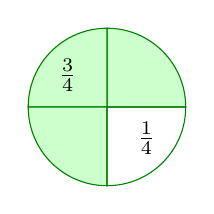
\begin{tikzpicture}
    \filldraw[fill=green!20,draw=green!50!black] (0,0) -- (1cm,0cm) arc [start angle=0, end angle=90, radius=1cm] -- cycle;
    \filldraw[fill=green!20,draw=green!50!black] (0,0) -- (0cm,1cm) arc [start angle=90, end angle=180, radius=1cm] -- cycle;
    \draw[fill=green!20,draw=green!50!black] (0,0) -- (-1cm,0cm) arc [start angle=180, end angle=270, radius=1cm] -- cycle;
    \draw[green!20,draw=green!50!black] (0,0) -- (0cm,-1cm) arc [start angle=270, end angle=360, radius=1cm] -- cycle;
    \node at (-0.5,0.4) {$\frac{3}{4}$};
    \node at (0.5,-0.4) {$\frac{1}{4}$};
    \end{tikzpicture}
    \end{figure}

    Si solo se utiliza una unidad, la fracción se llama \textbf{propia}; en el caso que acabamos de ver $3/4$ es una fracción propia en la cual el numerador es menor que el denominador y se dice que la fracción es menor que la unidad. Mientras que si se utiliza más de una unidad en su representación, esta se denomina fracción \textbf{impropia} y por supuesto resulta ser mayor que la unidad. Veamos un caso: representemos el número $5/3$. En este caso tomamos la unidad y la partimos en tres partes iguales, pero solo podemos tomar $3$ partes de esa unidad; se hace necesario entonces tomar otra unidad y partirla también en $3$ partes, de las cuales tomaremos $2$ para completar la fracción solicitada que se muestra en la figura \ref{fig:fraccion02}. En esa misma figura podemos ver que para representar la fracción se utilizó una unidad entera y $2/3$ de otra unidad; se puede escribir esta fracción como un número mixto $\frac{5}{3}=1\frac{2}{3}$ y se lee ``un entero dos tercios''.

    \begin{figure}[ht]
    \caption{Representación de la fracción impropia $5/3$}\label{fig:fraccion02}
    \centering
    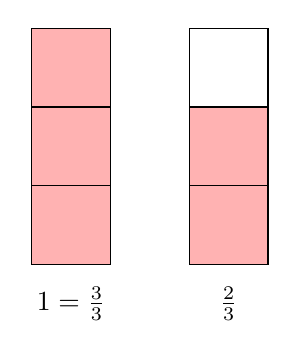
\begin{tikzpicture}
    \filldraw[red!30] (-2,-2) rectangle (-1,1);
    \draw (-2,-2) rectangle (-1,1);
    \draw (-2,-1)--(-1,-1);
    \draw (-2,0)--(-1,0);
    \filldraw[red!30] (0,-2) rectangle (1,-1);
    \draw (0,-2) rectangle (1,-1);
    \filldraw[red!30] (0,-1) rectangle (1,0);
    \draw (0,-1) rectangle (1,0);
    \draw (0,-2) rectangle (1,1);
    \node at (-1.5,-2.5) {$1=\frac{3}{3}$};
    \node at (0.5,-2.5) {$\frac{2}{3}$};
    \end{tikzpicture}
    \end{figure}

    Veamos que esto tiene relación directa con el algoritmo de Euclides, pues al hacer la división de $5$ entre $3$ se obtiene:
    \begin{center}
    \opidiv[displayintermediary=all, voperation=top]{5}{3}
    \end{center}
    Que lo escribimos como: 
    \[ \frac{5}{3}=1+\frac{2}{3} \]
    Una conclusión que podemos sacar de esta explicación es que si una unidad se divide en un número $b$ de partes y se toman $b$ partes, estamos tomando el equivalente a toda la unidad, así $\frac{3}{3}=1$, $\frac{5}{5}=1$. 

    \textbf{Propiedad de los racionales:} a cada racional $b\neq 0$ le corresponde otro racional $\frac{1}{b}$ tal que $b\cdot\frac{1}{b}=1$. Al número $\frac{1}{b}$ se le llama inverso multiplicativo del número $b$. En algunas ocasiones esto se escribe como la cancelación del número $b$ tanto en el numerador como en el denominador así $\cancel{b}\cdot{\frac{1}{\cancel{b}}}=1$. Así por ejemplo el inverso de $3$ es $\frac{1}{3}$ y cumple que $\cancel{3}\cdot\frac{1}{\not3}=1$, el inverso de $4$ es $\frac{1}{4}$ y cumple que $\cancel{4}\cdot\frac{1}{\not4}=1$, etc.

    \textbf{Representación sobre una recta:} Otra forma de representar los fraccionarios es sobre una recta infinita; se selecciona un punto arbitrario y se le asigna el número $0$, luego se selecciona un segmento (de cualquier longitud) que será nuestra unidad. Si por ejemplo queremos representar el fraccionario $1/2$ basta con dividir nuestra unidad en $2$ partes iguales y ubicar el segmento, allí estará el valor de la fracción, ver figura \ref{fig:fraccion03}.

    \begin{figure}[ht]
    \caption{Representación sobre una recta}\label{fig:fraccion03}
    \centering
    \begin{tikzpicture}
    \draw[->] (-1,0)--(2,0);
    \draw (0,0.1)--(0,-0.1);
    \node[below] at (0,0) {$0$};
    \draw (1,0.1)--(1,-0.1);
    \node[below] at (1,0) {$1$};
    \draw (0.5,0.1)--(0.5,-0.1);
    \node[above] at (0.5,0) {$\frac{1}{2}$};
    \end{tikzpicture}
    \end{figure}

    \item \textbf{Equivalencias:} los fraccionarios tienen distintas formas de escritura o de representación; en esta sección revisaremos algunas de esas representaciones equivalentes.

    \textbf{Fracciones equivalentes:} Una unidad se puede partir de distintas maneras. Así por ejemplo se puede representar el fraccionario $\frac{1}{2}$ partiendo la unidad en $2$ partes iguales y tomando una de esas partes como se puede apreciar en la figura \ref{fig:fraccion04}, pero al partir la misma unidad en $4$ partes iguales y tomar dos de esas partes se obtiene la misma región sombreada; el fraccionario equivalente es $\frac{2}{4}$, así podemos decir que $\frac{1}{2}=\frac{2}{4}$. Si partimos la unidad en $8$ partes y tomamos $4$ también podemos ver que representa la misma región sombreada, así $\frac{4}{8}=\frac{1}{2}$. En general diremos que dos fracciones son equivalentes si representan la misma región.

    \begin{figure}[ht]
    \caption{Fracciones Equivalentes a $\frac{1}{2}$}\label{fig:fraccion04}
    \centering
    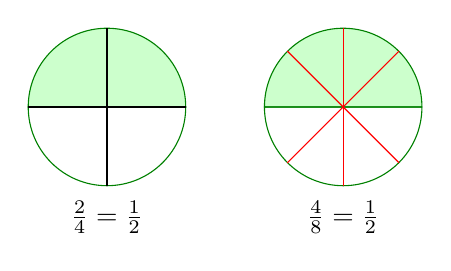
\begin{tikzpicture}
    \filldraw[fill=green!20,draw=green!50!black] (0,0) -- (1cm,0cm) arc [start angle=0, end angle=180, radius=1cm] -- cycle;
    \draw[green!20,draw=green!50!black] (0,0) -- (-1cm,0cm) arc [start angle=180, end angle=360, radius=1cm] -- cycle;
    \draw (0,0)--(0,1);
    \draw (0,0)--(-1,0);
    \draw (0,0)--(0,-1);
    \draw (0,0)--(1,0);
    \node at (0,-1.4) {$\frac{2}{4}=\frac{1}{2}$};
    
    \begin{scope}[shift={(3,0)}]
    \filldraw[fill=green!20,draw=green!50!black] (0,0) -- (1cm,0cm) arc [start angle=0, end angle=180, radius=1cm] -- cycle;
    \draw[green!20,draw=green!50!black] (0,0) -- (1cm,0cm) arc [start angle=0, end angle=-180, radius=1cm] -- cycle;
    \draw[red] (0,0)--(0.71,0.71);
    \draw[red] (0,0)--(0,1);
    \draw[red] (0,0)--(-0.71,0.71);
    \draw[red] (0,0)--(-0.71,-0.71);
    \draw[red] (0,0)--(0.0,-1.0);
    \draw[red] (0,0)--(0.71,-0.71);
    \node at (0,-1.4) {$\frac{4}{8}=\frac{1}{2}$};
    \end{scope}
    \end{tikzpicture}
    \end{figure}

    Es posible obtener fracciones equivalentes a una fracción dada si multiplicamos tanto el numerador como el denominador por una misma cantidad; las fracciones resultantes son equivalentes. A este proceso lo llamaremos \textbf{amplificación}, así por ejemplo: 
    \[ \frac{1}{2}=\frac{1\cdot 2}{2\cdot 2}=\frac{2}{4} \] 
    También lo podemos hacer por $4$ y resulta:
    \[ \frac{1}{2}=\frac{1\cdot 4}{2\cdot 4}=\frac{4}{8} \] 
    En realidad, podemos amplificar una fracción por cualquier número, resultando siempre una fracción equivalente.

    Para comprobar que dos fracciones digamos $\frac{a}{b}$ y $\frac{c}{d}$ son iguales, es posible hacer el producto cruzado: 
    \begin{equation}
    \frac{a}{b}=\frac{c}{d}\ \iff\ a\cdot d=c\cdot b 
    \end{equation}
    Así por ejemplo para determinar que $2/4$ equivale a $1/2$ podemos hacer $\frac{2}{4}=\frac{1}{2}$ y probar que $2\cdot 2=1\cdot 4=4$ y por tanto las fracciones son equivalentes.

    \textbf{Simplificación:} Cuando se tiene una fracción y tanto el numerador como el denominador se pueden escribir con su factorización prima, se pueden hacer las simplificaciones correspondientes y obtener una fracción equivalente a la fracción original. Así para el fraccionario $\frac{18}{24}$, descomponemos $18=2\cdot 3^2$ y $24=2^3\cdot 3$ y utilizando las propiedades de la potenciación resulta:
    \[ \frac{18}{24}=\frac{\cancel{2}\cdot 3^{\not2}}{2^{\not3}\cdot \cancel{3}}=\frac{3}{4} \]
    Que son equivalentes, pues al multiplicar en cruz se obtiene $18\cdot 4=72=3\cdot 24$.

    Al representar las fracciones sobre una recta, se está diciendo que el punto $1/2$ también se puede escribir como $\frac{\textcolor{red}{1}}{\textcolor{red}{2}}=\frac{\textcolor{blue}{2}}{\textcolor{blue}{4}}=\frac{\textcolor{brown}{3}}{\textcolor{brown}{6}}=\cdots$, como se puede ver en la figura \ref{fig:fraccion05}.

    \begin{figure}[ht]
    \caption{Fracciones Equivalentes}\label{fig:fraccion05}
    \centering
    \begin{tikzpicture}
    \draw[->] (-1,0)--(4,0);
    \draw (0,0.1)--(0,-0.1);
    \node[below] at (0,0) {$0$};
    \draw (2,0.1)--(2,-0.1);
    \node[below] at (2,0) {$1$};
    \draw (1,0.1)--(1,-0.1);
    \node at (1,0) {$\bullet$}; 
    \node at (1,0.5) {$\frac{\textcolor{red}{1}}{\textcolor{red}{2}}$};
    \node at (1,-0.5) {$\frac{\textcolor{blue}{2}}{\textcolor{blue}{4}}$};
    \node at (1,-1.1) {$\frac{\textcolor{brown}{3}}{\textcolor{brown}{6}}$};
    \node at (1,-1.6) {$\vdots$};
    \end{tikzpicture}
    \end{figure}

    Lo que indica que un punto sobre la recta tiene una cantidad infinita de representaciones.

\textbf{Representación Decimal:} Al dividir un número entero entre otro, existen dos posibilidades para el cociente: que sea un número entero (división exacta, ej. $12 \div 4 = 3$) o que no lo sea. En este último caso, entramos al dominio de los números racionales con expansión decimal.

Consideremos la división $\frac{11}{4}$. Al realizar el algoritmo usual, vemos que $4$ cabe $2$ veces en $11$ y sobra un residuo de $3$. En los números enteros ahí terminaría el proceso. Sin embargo, en los racionales podemos continuar:

\begin{enumerate}
    \item Como el residuo $3$ es menor que el divisor $4$, colocamos una \textbf{coma decimal} en el cociente.
    \item Esto nos permite transformar el residuo: convertimos las 3 unidades sobrantes en 30 \textit{décimas}.
    \item Ahora dividimos $30$ entre $4$, lo que nos da $7$ (décimas) y sobra un nuevo residuo de $2$.
    \item Repetimos el proceso agregando otro cero (convirtiendo el 2 en 20 \textit{centésimas}).
\end{enumerate}

Este proceso se ilustra paso a paso en la Figura \ref{fig:divisiondecimal03}.

  \begin{figure}[ht]
\begin{center}
\caption{División con Decimales}\label{fig:divisiondecimal03}
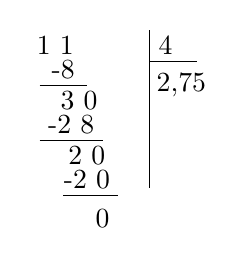
\begin{tikzpicture}[domain=-2:1,scale=1]
\draw (0.2,0.0) -- (0.2,-2.0);
\draw (-1.0,-0.2) node{1 1};
\draw (0.4,-0.2) node{4};
\draw (0.2,-0.4) -- (0.8,-0.4);
\draw (0.6,-0.7) node{2,75};
\draw (-0.9,-0.5) node{-8};
\draw (-1.2,-0.7) -- (-0.6,-0.7);
\draw (-0.7,-0.9) node{3 0};
\draw (-0.8,-1.2) node{-2 8};
\draw (-1.2,-1.4)--(-0.4,-1.4);
\draw (-0.6,-1.6) node {2 0};
\draw (-0.6,-1.9) node {-2 0};
\draw (-0.9,-2.1)--(-0.2,-2.1);
\draw (-0.4,-2.4) node {0};
\end{tikzpicture}
\end{center}  
 \end{figure}
Al llegar a un residuo de cero, el proceso termina. Concluimos que $\frac{11}{4} = 2,75$. A este tipo de número se le llama \textbf{decimal finito} o exacto.

Por otro lado, existen divisiones donde el residuo nunca se hace cero, sino que empieza a repetirse. Por ejemplo, al dividir $\frac{2}{3}$ obtenemos $0,666\dots$. En este caso, usamos una barra sobre la parte que se repite (el periodo) y escribimos $\frac{2}{3}=0,\overline{6}$. A estos se les llama \textbf{decimales infinitos periódicos}.

En resumen, podemos caracterizar formalmente al conjunto de los números racionales $\mathbb{Q}$ de la siguiente manera:

\begin{align}
    \mathbb{Q} &= \left\{\frac{a}{b} \mid a,b\in\mathbb{Z}, b\neq 0\right\} \\
               &= \{\text{Números con expansión decimal finita o infinita periódica}\}
\end{align}

\textit{Nota:} Todo número entero es también un número racional, ya que cualquier $m \in \mathbb{Z}$ puede escribirse como $\frac{m}{1}$.


\textbf{Porcentajes:} Los porcentajes son una forma estandarizada de representar partes de un todo utilizando como base el número 100. Formalmente, el símbolo \% representa al factor $\frac{1}{100}$.

Por ejemplo, sabemos que la fracción $\frac{1}{2}$ equivale al decimal $0,5$. Si queremos expresarlo como porcentaje, buscamos una fracción equivalente con denominador 100:
\[ 0,5 = \frac{5}{10} = \frac{50}{100} = 50 \cdot \frac{1}{100} = 50\% \]
Esto se lee como ``cincuenta por ciento''.


\textbf{Cálculo de porcentajes:} Para hallar el porcentaje de una cantidad, interpretamos el porcentaje como un operador multiplicativo. Por ejemplo, calcular el $50\%$ \textbf{de} $20$ objetos equivale a:
\[ 50\% \cdot 20 = \frac{50}{100} \cdot 20 = 0,5 \cdot 20 = 10 \]
Es decir, el $50\%$ de $20$ son $10$ unidades (la mitad). La Figura \ref{fig:porcentaje100} ilustra gráficamente cómo el $1\%$ corresponde a un solo cuadro de una cuadrícula de cien.

\begin{figure}[ht]
    \centering
    \caption{Interpretación gráfica del Porcentaje}
    \label{fig:porcentaje100}
    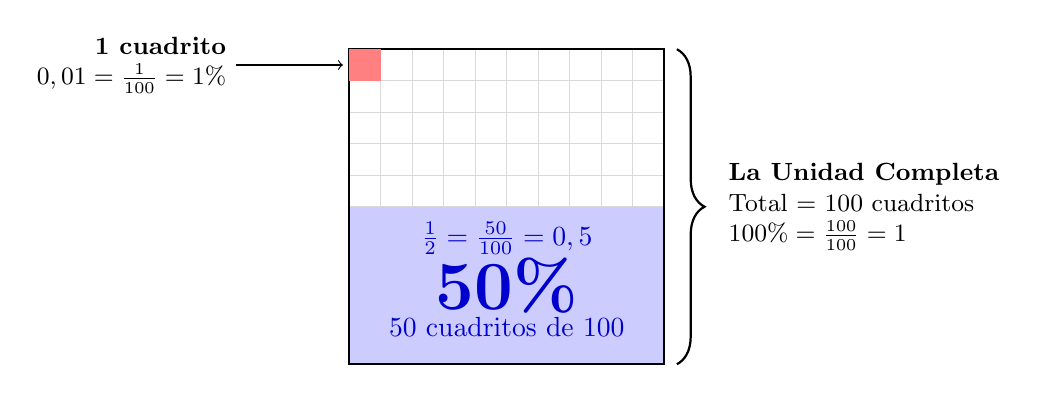
\begin{tikzpicture}[scale=0.8]
        % 1. La Cuadrícula base (10x10)
        % Dibujamos 100 cuadritos en gris muy suave
        \draw[step=0.5cm, gray!30, thin] (0,0) grid (5,5);
        
        % 2. Sombreado del 50% (50 cuadritos)
        % Llenamos la mitad inferior de azul suave
        \fill[blue!20] (0,0) rectangle (5,2.5);
        
        % 3. Borde grueso del TOTAL (El 100%)
        \draw[thick, black] (0,0) rectangle (5,5);
        
        % --- ANOTACIONES ---
        
        % Explicación de 1% (Un solo cuadrito)
        % CORREGIDO: 0.01 es el valor correcto, no 0.1
        \fill[red!50] (0,4.5) rectangle (0.5,5); 
        \draw[<-] (-0.1, 4.75) -- (-1.8, 4.75) node[left, align=right, font=\small] {\textbf{1 cuadrito}\\ $0,01=\frac{1}{100} = 1\%$};
        
        % Explicación del 50% (Área azul)
        \node[blue!80!black] at (2.5, 1.25) {\Huge \textbf{50\%}};
        \node[blue!80!black] at (2.5, 0.6) {50 cuadritos de 100};
        \node[blue!80!black] at (2.5, 2.0) {$\frac{1}{2}=\frac{50}{100} = 0,5$};
        
        % Explicación del 100% (Llave lateral)
        % Requiere \usetikzlibrary{decorations.pathreplacing} en el preámbulo
        \draw[decorate, decoration={brace, amplitude=10pt, mirror}, thick] (5.2, 0) -- (5.2, 5) 
            node[midway, right=15pt, align=left, font=\small] {\textbf{La Unidad Completa}\\ Total = 100 cuadritos\\ $100\% = \frac{100}{100} = 1$};
    \end{tikzpicture}
\end{figure}
    \item \textbf{Suma de Fraccionarios:} a continuación se presentan diversas opciones para realizar la suma de fracciones, dependiendo de si son \textbf{homogéneas} (mismo denominador) o \textbf{heterogéneas} (denominador distinto).

    \begin{enumerate}
        \item \textbf{Suma de Fracciones Homogéneas:} si tienen el mismo denominador, se suman los numeradores y se deja el mismo denominador:
        \begin{equation}
        \boxed{\frac{a}{b}+\frac{c}{b}=\frac{a+c}{b}}
        \end{equation}
        Por ejemplo: 
        \[ \frac{2}{5}+\frac{4}{5}=\frac{6}{5} \]

        \item \textbf{Suma de Fracciones Heterogéneas:} dadas dos fracciones con diferente denominador hay varias formas para realizar su suma:
        
        \textbf{Multiplicación en Cruz:}
        \begin{equation}
        \boxed{\frac{a}{b}+\frac{c}{d}=\frac{ad+bc}{bd}}
        \end{equation}
        Ejemplo:
        \[ \frac{3}{\textcolor{red}{4}}+\frac{\textcolor{brown}{2}}{\textcolor{blue}{5}}=\frac{3\cdot \textcolor{blue}{5}+\textcolor{brown}{2}\cdot \textcolor{red}{4}}{\textcolor{red}{4}\cdot \textcolor{blue}{5}}=\frac{15+8}{20}=\frac{23}{20} \]

        \textbf{Amplificando las fracciones:} para dejarlas con el mismo denominador.
        \[ \frac{2}{3}+4=\frac{2}{3}+\frac{4}{1}\cdot\frac{3}{3}=\frac{2}{3}+\frac{12}{3}=\frac{14}{3} \]

        \textbf{Utilizando el MCM:} Sumar $\frac{7}{90}$ con $\frac{13}{120}$. 
        $\mathcal{MCM}(90,120)=360$.
        \begin{equation*}
            \frac{7}{90}+\frac{13}{120}=\frac{7\cdot 4+13\cdot 3}{360}=\frac{28+39}{360}=\frac{67}{360}
        \end{equation*}
    \end{enumerate}
%===============================================================
\item \textbf{Multiplicación de Fraccionarios:} 
    Conceptualmente, multiplicar fracciones significa calcular una parte de otra parte. La palabra clave es ``\textbf{de}''.
    
    El algoritmo es directo: numerador por numerador y denominador por denominador.
    \begin{equation}
    \boxed{\frac{a}{b} \cdot \frac{c}{d} = \frac{a \cdot c}{b \cdot d}}
    \end{equation}
    \textbf{Ejemplo Numérico:} Multiplicar $\frac{2}{3}$ por $\frac{4}{5}$:
    \[ \frac{2}{3} \cdot \frac{4}{5} = \frac{2 \cdot 4}{3 \cdot 5} = \frac{8}{15} \]

    \textbf{Explicación Gráfica (Paso a paso):} 
    Vamos a visualizar la operación $\frac{2}{3} \cdot \frac{4}{5}$ (que se lee: ``dos tercios \textbf{de} cuatro quintos'') ver figura \ref{fig:multpasos}.
    
       \begin{figure}[ht]
    \centering
    \caption{Proceso gráfico de multiplicación con rejilla}\label{fig:multpasos}
    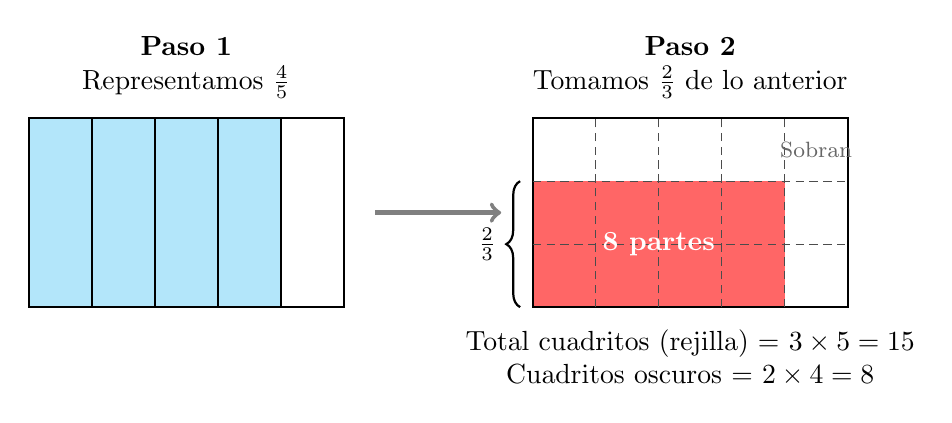
\begin{tikzpicture}[scale=0.8]
        % --- PASO 1: Representar 4/5 ---
        \node[align=center] at (2.5, 3.8) {\textbf{Paso 1}\\Representamos $\frac{4}{5}$};
        % Relleno Azul
        \fill[cyan!30] (0,0) rectangle (4,3);
        % Borde Unidad
        \draw[thick] (0,0) rectangle (5,3);
        % Divisiones Verticales (Quintos) - Sólidas
        \foreach \x in {1,2,3,4} \draw[thick] (\x,0) -- (\x,3);
        
        % Flecha de transición
        \draw[->, ultra thick, gray] (5.5, 1.5) -- (7.5, 1.5);

        % --- PASO 2: Cruzar con 2/3 y ver la rejilla ---
        \begin{scope}[shift={(8,0)}]
            \node[align=center] at (2.5, 3.8) {\textbf{Paso 2}\\Tomamos $\frac{2}{3}$ de lo anterior};
            
            % 1. Relleno Final (Intersección) - Más oscuro para destacar
            \fill[red!60] (0,0) rectangle (4,2);
            
            % 2. Borde Unidad
            \draw[thick] (0,0) rectangle (5,3);
            
            % 3. LA REJILLA COMPLETA (Líneas punteadas para visualizar el total)
            % Verticales (Quintos)
            \foreach \x in {1,2,3,4} \draw[densely dashed, black!70] (\x,0) -- (\x,3);
            % Horizontales (Tercios)
            \foreach \y in {1,2} \draw[densely dashed, black!70] (0,\y) -- (5,\y);
            
            % Etiquetas explicativas
            \draw[decorate, decoration={brace, amplitude=5pt}, thick] (-0.2, 0) -- (-0.2, 2) 
                node[midway, left=5pt] {$\frac{2}{3}$};
                
            \node[white, font=\bfseries] at (2,1) {8 partes};
            \node[black!60, font=\footnotesize] at (4.5, 2.5) {Sobran};
            
            % Conteo visual abajo
            \node[below, align=center] at (2.5, -0.2) {
                Total cuadritos (rejilla) = $3 \times 5 = 15$ \\
                Cuadritos oscuros = $2 \times 4 = 8$
            };
        \end{scope}
    \end{tikzpicture}
    \end{figure}
 
    \begin{enumerate}
        \item En el \textbf{Paso 1}, dividimos la unidad verticalmente en 5 partes y tomamos 4 (zona azul).
        \item En el \textbf{Paso 2}, dividimos horizontalmente en 3 partes y seleccionamos 2 filas (zona roja).
        \item El resultado es la zona roja, que contiene $4 \times 2 = 8$ cuadros.
        \item El total de cuadros en la rejilla nueva es $5 \times 3 = 15$.
    \end{enumerate}
    
    Por lo tanto:
    \[ \frac{2}{3} \cdot \frac{4}{5} = \frac{8}{15} \]



    \textbf{Ejemplo Numérico:} Multiplicar $\frac{3}{4}$ por $\frac{5}{7}$:
    \[ \frac{3}{4} \cdot \frac{5}{7} = \frac{3 \cdot 5}{4 \cdot 7} = \frac{15}{28} \]

%===============================================================
    
    \textbf{Recomendación (Simplificación previa):} En la multiplicación es muy útil simplificar cualquier numerador con cualquier denominador \textit{antes} de multiplicar, para evitar trabajar con números muy grandes.
    
    \textbf{Ejemplo con simplificación:} Multiplicar $\frac{4}{9} \cdot \frac{3}{10}$.
    \[ \frac{\textcolor{red}{4}}{\textcolor{blue}{9}} \cdot \frac{\textcolor{blue}{3}}{\textcolor{red}{10}} = \frac{\cancelto{2}{4} \cdot \cancelto{1}{3}}{\cancelto{3}{9} \cdot \cancelto{5}{10}} = \frac{2 \cdot 1}{3 \cdot 5} = \frac{2}{15} \]
    En este caso, simplificamos el 4 con el 10 (sacando mitad) y el 3 con el 9 (sacando tercera).
    
 \item \textbf{División de Fraccionarios:} 
    Conceptualmente, la división $\frac{a}{b} \div \frac{c}{d}$ responde a la pregunta: \textbf{¿Cuántas veces cabe la fracción $\frac{c}{d}$ dentro de la fracción $\frac{a}{b}$?}
    
    Existen dos métodos mecánicos principales para resolverla:
    
    \textbf{Método 1: Invertir y Multiplicar.} Se multiplica la primera fracción (dividendo) por el \textbf{inverso multiplicativo} de la segunda fracción (divisor).
    \begin{equation}
    \boxed{\frac{a}{b} \div \frac{c}{d} = \frac{a}{b} \cdot \frac{d}{c} = \frac{a \cdot d}{b \cdot c}}
    \end{equation}
    
    \textbf{Explicación Gráfica (El concepto de cabida):}
    Vamos a visualizar la división $\frac{3}{4} \div \frac{1}{8}$.
    
    Matemáticamente, aplicando la fórmula:
    \[ \frac{3}{4} \div \frac{1}{8} = \frac{3}{4} \cdot \frac{8}{1} = \frac{24}{4} = 6 \]
    Esto nos dice que $\frac{1}{8}$ cabe exactamente \textbf{6 veces} en $\frac{3}{4}$. Veámoslo:

        \begin{figure}[ht]
    \centering
    \caption{Visualización de $\frac{3}{4} \div \frac{1}{8}$ (¿Cuántos octavos caben?)}\label{fig:divfrac}
    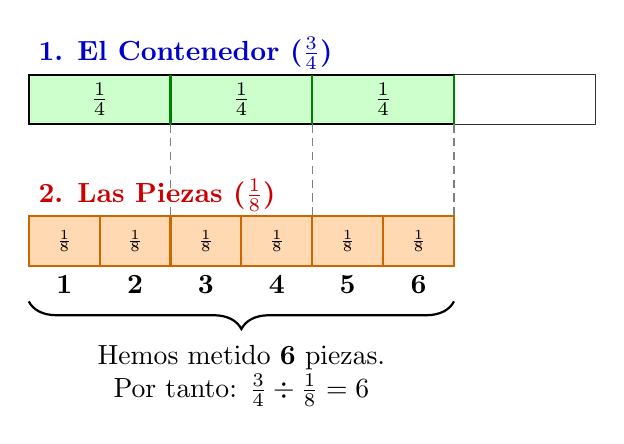
\begin{tikzpicture}[scale=0.9]
        % --- ESCALA: 8 unidades de ancho = 1 Entero ---
        
        % --- NIVEL 1: EL CONTENEDOR (3/4) ---
        \node[anchor=west, blue!80!black] at (0, 3.5) {\textbf{1. El Contenedor ($\frac{3}{4}$)}};
        
        % La Unidad completa fantasma (para referencia)
        \draw[black!80] (0,2.5) rectangle (8,3.2);
        
        % El 3/4 relleno
        \fill[green!20] (0,2.5) rectangle (6,3.2);
        \draw[thick] (0,2.5) rectangle (6,3.2);
        
        % Divisiones de cuartos
        \foreach \x in {2,4,6} \draw[thick, green!50!black] (\x,2.5) -- (\x,3.2);
        
        % Etiquetas de cuartos
        \node at (1, 2.85) {$\frac{1}{4}$};
        \node at (3, 2.85) {$\frac{1}{4}$};
        \node at (5, 2.85) {$\frac{1}{4}$};
        
        % --- LÍNEAS GUÍA (Muestran que 1/4 = 2/8) ---
        \foreach \x in {2,4,6} \draw[densely dashed, gray] (\x, 2.5) -- (\x, 1.2);

        % --- NIVEL 2: LAS PIEZAS (1/8) ---
        \node[anchor=west, red!80!black] at (0, 1.5) {\textbf{2. Las Piezas ($\frac{1}{8}$)}};
        
        % Dibujamos las 6 cajitas que caben
        \foreach \i in {0,1,2,3,4,5} {
            % Caja naranja
            \fill[orange!30] (\i,0.5) rectangle (\i+1,1.2);
            \draw[thick, orange!80!black] (\i,0.5) rectangle (\i+1,1.2);
            % Texto pequeño dentro
            \node[font=\tiny] at (\i+0.5, 0.85) {$\frac{1}{8}$};
            % Número de conteo abajo
            \node[font=\bfseries, below] at (\i+0.5, 0.5) {\number\numexpr\i+1};
        }
        
        % --- NIVEL 3: CONCLUSIÓN ---
        \draw[decorate, decoration={brace, amplitude=10pt, mirror}, thick] (0, 0) -- (6, 0) 
            node[midway, below=12pt, align=center] {
                Hemos metido \textbf{6} piezas.\\
                Por tanto: $\frac{3}{4} \div \frac{1}{8} = 6$
            };
            
    \end{tikzpicture}
    \end{figure}

    \textbf{Ejemplo General:} Para $\frac{2}{3} \div \frac{5}{7}$, aplicamos la regla:
    \[ \frac{2}{3} \div \frac{5}{7} = \frac{2}{3} \cdot \frac{7}{5} = \frac{14}{15} \]

    \textbf{Método 2: Ley de la Oreja (Producto de extremos y medios).} Se organiza la división como una ``fracción de fracciones''. El resultado es el producto de los extremos (los números de más arriba y más abajo) sobre el producto de los medios (los números internos).
    %==========================================================
        \begin{figure}[ht]
    \centering
    \begin{tikzpicture}
       \node (A) at (0,1.2) {$a$};
       \node (B) at (0,0.6) {$b$};
       \draw (A.south west) -- (A.south east); 
       
       \node (C) at (0,-0.6) {$c$};
       \node (D) at (0,-1.2) {$d$};
       \draw (C.south west) -- (C.south east); 
       
       \draw[thick] (-0.5,0) -- (0.5,0); 
       
       % CAMBIO CLAVE AQUÍ:
       % 'pos=0.1' pone el texto arriba (al inicio de la curva roja)
       \draw[red, ->] (A.east) to[bend left=80] node[pos=0.3, right] {Extremos ($a \cdot d$)} (D.east);
       
       % 'pos=0.9' pone el texto abajo (al final de la curva azul)
       \draw[blue, ->] (B.east) to[bend left=80] node[pos=0.9, right] {Medios ($b \cdot c$)} (C.east);
       
       \node at (5,0) {$= \dfrac{a \cdot d}{b \cdot c}$};
    \end{tikzpicture}
    \caption{Ley de la Oreja}\label{fig:leyoreja}
    \end{figure}


    %==========================================================    
    \textbf{Ejemplo:} $\dfrac{\frac{1}{2}}{\frac{3}{5}} = \frac{1 \cdot 5}{2 \cdot 3} = \frac{5}{6}$.
    
\end{enumerate}

\subsection*{Ejemplos Resueltos Adicionales}

\textbf{Ejemplo 1: Simplificación de Fracciones} \\
Simplifique la fracción $\frac{84}{126}$ hasta su mínima expresión.

\textit{Solución:}
Descomponemos el numerador y el denominador en factores primos:
$84 = 2^2 \cdot 3 \cdot 7$ y $126 = 2 \cdot 3^2 \cdot 7$.
Sustituimos y cancelamos los factores comunes:
\[ \frac{84}{126} = \frac{2^2 \cdot 3 \cdot 7}{2 \cdot 3^2 \cdot 7} = \frac{2}{3} \]

\vspace{0.3cm}

\textbf{Ejemplo 2: De Decimal Periódico a Fracción} \\
Convierta el decimal infinito periódico $0,333\dots$ (es decir, $0,\overline{3}$) a una fracción.

\textit{Solución:}
Sea $x = 0,333\dots$.
Multiplicamos por $10$ a ambos lados (para mover la coma un lugar):
\[ 10x = 3,333\dots \]
Restamos la ecuación original ($x = 0,333\dots$) a esta nueva ecuación:
\begin{align*}
    10x &= 3,333\dots \\
    - x &= 0,333\dots \\
    \hline
    9x &= 3
\end{align*}
Despejamos $x$:
\[ x = \frac{3}{9} = \frac{1}{3} \]

\subsection*{Ejercicios Propuestos}

\begin{enumerate}
    \item \textbf{Operaciones básicas:}
    Realice las siguientes sumas y simplifique el resultado.
    \begin{enumerate}
        \item $\frac{3}{8} + \frac{1}{8}$
        \item $\frac{2}{5} + \frac{1}{3}$
        \item $\frac{5}{12} + \frac{7}{18}$
    \end{enumerate}
    
    \item \textbf{Equivalencia:}
    Determine si las siguientes parejas de fracciones son equivalentes justificando su respuesta (ya sea simplificando o multiplicando en cruz).
    \begin{enumerate}
        \item $\frac{3}{5}$ y $\frac{9}{15}$
        \item $\frac{4}{7}$ y $\frac{12}{20}$
    \end{enumerate}

    \item \textbf{Orden y densidad :}
    Encuentre una fracción que cumpla las siguientes dos condiciones simultáneamente:
    \begin{itemize}
        \item Que su denominador sea exactamente 12.
        \item Que sea mayor que $\frac{1}{3}$ pero menor que $\frac{1}{2}$.
    \end{itemize}
    \textit{Pista: Convierta los límites a fracciones con denominador 12.}

    \item \textbf{Problema del Tanque:}
    Un tanque se llena hasta sus $3/4$ partes de capacidad. Si luego se extrae una cantidad de agua equivalente a $1/5$ de la \textbf{capacidad total} del tanque, ¿qué fracción del tanque queda llena?

    \item \textbf{Lógica de Porcentajes :}
    Sin usar calculadora, determine qué cantidad es mayor o si son iguales:
    \begin{itemize}
        \item El $28\%$ de $50$.
        \item El $50\%$ de $28$.
    \end{itemize}
    Justifique su respuesta algebraicamente probando si $x\%$ de $y$ es igual a $y\%$ de $x$.

    \item \textbf{Variaciones porcentuales sucesivas:}
    El precio de un artículo sube un $10\%$ en enero. En febrero, el nuevo precio baja un $10\%$. ¿El precio final es igual, mayor o menor que el precio original antes de enero? Demuestre su respuesta asumiendo un precio inicial $P$.

    \item \textbf{Patrones en decimales :}
    La fracción $\frac{1}{7}$ tiene un desarrollo decimal periódico:
    \[ \frac{1}{7} = 0,142857142857\dots \]
    Sin hacer la división completa, determine cuál es el dígito que ocupa la posición número 100 después de la coma.
    \textit{Sugerencia: Analice la longitud del periodo y use la aritmética modular (el residuo de dividir 100 entre la longitud).}

    \item \textbf{Falsos promedios :}
    Un ciclista sube una montaña a una velocidad de $10$ km/h y la baja a una velocidad de $30$ km/h. ¿Cuál es su velocidad promedio para el viaje completo?
    \textit{Nota: La respuesta no es $20$ km/h. Defina la distancia como $d$ y utilice la fórmula $t = d/v$.}
\end{enumerate}
